\documentclass[12pt]{article}
\usepackage{graphicx,import}
\usepackage[svgnames]{xcolor} 
\usepackage{fancyhdr}
\usepackage{subfig}
\usepackage{hyperref}
\usepackage{enumitem}
\usepackage{cite}
\usepackage{fancyvrb}
\usepackage[many]{tcolorbox}
\usepackage{listings }
\usepackage[a4paper, total={6in, 8in} , bottom = 25mm , top = 25mm, headheight = 1.25cm , includehead,includefoot,heightrounded ]{geometry}
\usepackage{afterpage}
\usepackage{amssymb}
\usepackage{pdflscape}
\usepackage{gensymb}
\usepackage{textcomp}
\usepackage{tikz,pgfplots}
\usepackage{xecolor}
\usepackage{rotating}
\usepackage{pdfpages}
\usepackage[Kashida]{xepersian}
\usepackage[T1]{fontenc}
\usepackage{tikz}
\usepackage[utf8]{inputenc}
\usepackage{PTSerif} 
\usepackage{seqsplit}

\usepackage[edges]{forest}

\usepackage{listings}
\usepackage{xcolor}

\hypersetup{
	colorlinks   = true, %Colours links instead of ugly boxes
	urlcolor     = blue, %Colour for external hyperlinks
	linkcolor    = blue, %Colour of internal links
	citecolor   = red %Colour of citations
}
 
\definecolor{codegreen}{rgb}{0,0.6,0}
\definecolor{codegray}{rgb}{0.5,0.5,0.5}
\definecolor{codepurple}{rgb}{0.58,0,0.82}
\definecolor{backcolour}{rgb}{0.95,0.95,0.92}
 
\NewDocumentCommand{\codeword}{v}{
\texttt{\textcolor{blue}{#1}}
}
\lstset{language=java,keywordstyle={\bfseries \color{blue}}}

\lstdefinestyle{mystyle}{
    backgroundcolor=\color{backcolour},   
    commentstyle=\color{codegreen},
    keywordstyle=\color{magenta},
    numberstyle=\tiny\color{codegray},
    stringstyle=\color{codepurple},
    basicstyle=\ttfamily\normalsize,
    breakatwhitespace=false,         
    breaklines=true,                 
    captionpos=b,                    
    keepspaces=true,                 
    numbers=left,                    
    numbersep=5pt,                  
    showspaces=false,                
    showstringspaces=false,
    showtabs=false,                  
    tabsize=2
}

\lstset{style=mystyle}

\settextfont[Scale=1.2 ,BoldFont={Bahij Nazanin-Bold.ttf} , ItalicFont = {IRNazaninIranic.ttf}]{Bahij Nazanin-Regular.ttf}
\setlatintextfont[Scale = 1.0]{Garamond}
\DefaultMathsDigits 
\DeclareMathSizes{11}{19}{13}{9} 
%\DeclareMathSizes{12}{14.4}{8}{9}





\newenvironment{changemargin}[2]{%
\begin{list}{}{%
\setlength{\topsep}{0pt}%
\setlength{\leftmargin}{#1}%
\setlength{\rightmargin}{#2}%
\setlength{\listparindent}{\parindent}%
\setlength{\itemindent}{\parindent}%
\setlength{\parsep}{\parskip}%
}%
\item[]}{\end{list}}


\definecolor{foldercolor}{RGB}{124,166,198}

\tikzset{pics/folder/.style={code={%
    \node[inner sep=0pt, minimum size=#1](-foldericon){};
    \node[folder style, inner sep=0pt, minimum width=0.3*#1, minimum height=0.6*#1, above right, xshift=0.05*#1] at (-foldericon.west){};
    \node[folder style, inner sep=0pt, minimum size=#1] at (-foldericon.center){};}
    },
    pics/folder/.default={20pt},
    folder style/.style={draw=foldercolor!80!black,top color=foldercolor!40,bottom color=foldercolor}
}

\forestset{is file/.style={edge path'/.expanded={%
        ([xshift=\forestregister{folder indent}]!u.parent anchor) |- (.child anchor)},
        inner sep=1pt},
    this folder size/.style={edge path'/.expanded={%
        ([xshift=\forestregister{folder indent}]!u.parent anchor) |- (.child anchor) pic[solid]{folder=#1}}, inner xsep=0.6*#1},
    folder tree indent/.style={before computing xy={l=#1}},
    folder icons/.style={folder, this folder size=#1, folder tree indent=3*#1},
    folder icons/.default={12pt},
}

\begin{document}


%%% title pages
\begin{titlepage}
\begin{center}
        
\vspace*{0.7cm}


\includegraphics[width=0.4\textwidth]{sharif1.png}\\
\vspace{0.5cm}
\textbf{ \Huge{\emph ‌سیگنال‌ها و سیستم‌ها} }\\
\vspace{0.5cm}
\textbf{ \Large{ تمرین پنجم} }
\vspace{0.2cm}
       
 
      \large \textbf{دانشکده مهندسی کامپیوتر}\\\vspace{0.2cm}
    \large   دانشگاه صنعتی شریف\\\vspace{0.2cm}
       \large   ﻧﯿﻢ سال دوم 00-99 \\\vspace{0.2cm}
      \noindent\rule[1ex]{\linewidth}{1pt}
استاد:\\
    \textbf{{جناب آقای دکتر منظوری شلمانی}}


    \vspace{0.15cm}
نام و نام خانوادگی:\\

       
    \textbf{{امیرمهدی نامجو - 97107212}}
\end{center}
\end{titlepage}
%%% title pages


%%% header of pages
\newpage
\pagestyle{fancy}
\fancyhf{}
\fancyfoot{}
\cfoot{\thepage}
\chead{تمرین پنجم}
\rhead{
\includegraphics[width=0.1\textwidth]{sharif.png}}
\lhead{امیرمهدی نامجو}
%%% header of pages

\KashidaOff

\section{سری فوریه}
\subsection{سوال اول}

\subsubsection{بخش a}


$$
f(x)=\left\{\begin{array}{lr}
	\pi-x & 0 \leq x \leq \pi \\
	x-\pi & -\pi \leq x \leq 0
\end{array}\right.
$$

ابتدا عامل DC را بدست می‌آوریم:

$$a_0 = \frac{1}{2\pi} \int f(x) dx = \frac{1}{2\pi} \int_{-\pi}^{0} (x- \pi) dx + \int_{0}^{\pi} (\pi -x) dx$$
$$= \frac{1}{2\pi} (\frac{-3\pi^2}{2} - \frac{\pi^2}{2}) = \boxed{- \pi} $$

برای ضرایب کسینوسی داریم:

$$a_n = \frac{1}{\pi} \int (f(x) \cos (nx)) dx$$

$$= \frac{1}{\pi} (\int_{-\pi}^{0} (x - \pi) \cos (nx) dx + \int_{0}^{\pi} (\pi - x) \cos (nx) dx)$$

ابتدا لازم است اشاره کنیم که
$$\int x \cos (nx) = \frac{1}{n^2} \cos(nx) + \frac{1}{n} x \sin (nx)$$

با توجه به این موضوع، از عبارت بالا می‌توان به راحتی انتگرال گرفت:


$$= \frac{1}{\pi}( (\frac{\cos (n x)}{n^2}+\frac{x \sin (n x)}{n}-\frac{\pi  \sin (n x)}{n}) |_{-\pi}^{0} + (-\frac{\cos (n x)}{n^2}+\frac{\pi  \sin (n x)}{n}-\frac{x \sin (n x)}{n})|_{0}^{\infty})$$

بعد از ساده سازی و محاسبات داریم:

$$\boxed{a_n = -\frac{2 (\pi  n \sin (\pi  n)+\cos (\pi  n)-1)}{\pi  n^2}}$$


برای محاسبات ضریب سینوسی داریم:

$$b_n = \frac{1}{\pi} \int (f(x) sin(nx)) dx$$

$$= \frac{1}{\pi} (\int_{-\pi}^{0} (x - \pi) \sin (nx) dx + \int_{0}^{\pi} (\pi - x) \sin (nx) dx)$$


ابتدا لازم است اشاره کنیم که
$$\int x \sin(nx) = \frac{\sin (n x)}{n^2}-\frac{x \cos (n x)}{n} $$

با توجه به این موضوع، عبارت بالا مانند بخش قبل به راحتی قابل محاسبه است. جوابی که در نهایت به آن می رسیم به صورت زیر است:


$$\boxed{b_n = \frac{2-2 \cos (\pi  n)}{n}}$$


و جواب نهایی به صورت:

$$f(x) = a_0 + \sum_{n=1}^{N} (a_n \cos (n x) + b_n \sin (n x))$$

خواهد بود.

کد آن در فایل 
\lr{\Verb+P1\_Q1\_a.py+}
قرار دارد. نمودار در صفحه بعد قرار گرفته است. شکل بالایی خود تابع و شکل های بعدی به ازای $N=2,5,20,50$ هستند.

\begin{center}
	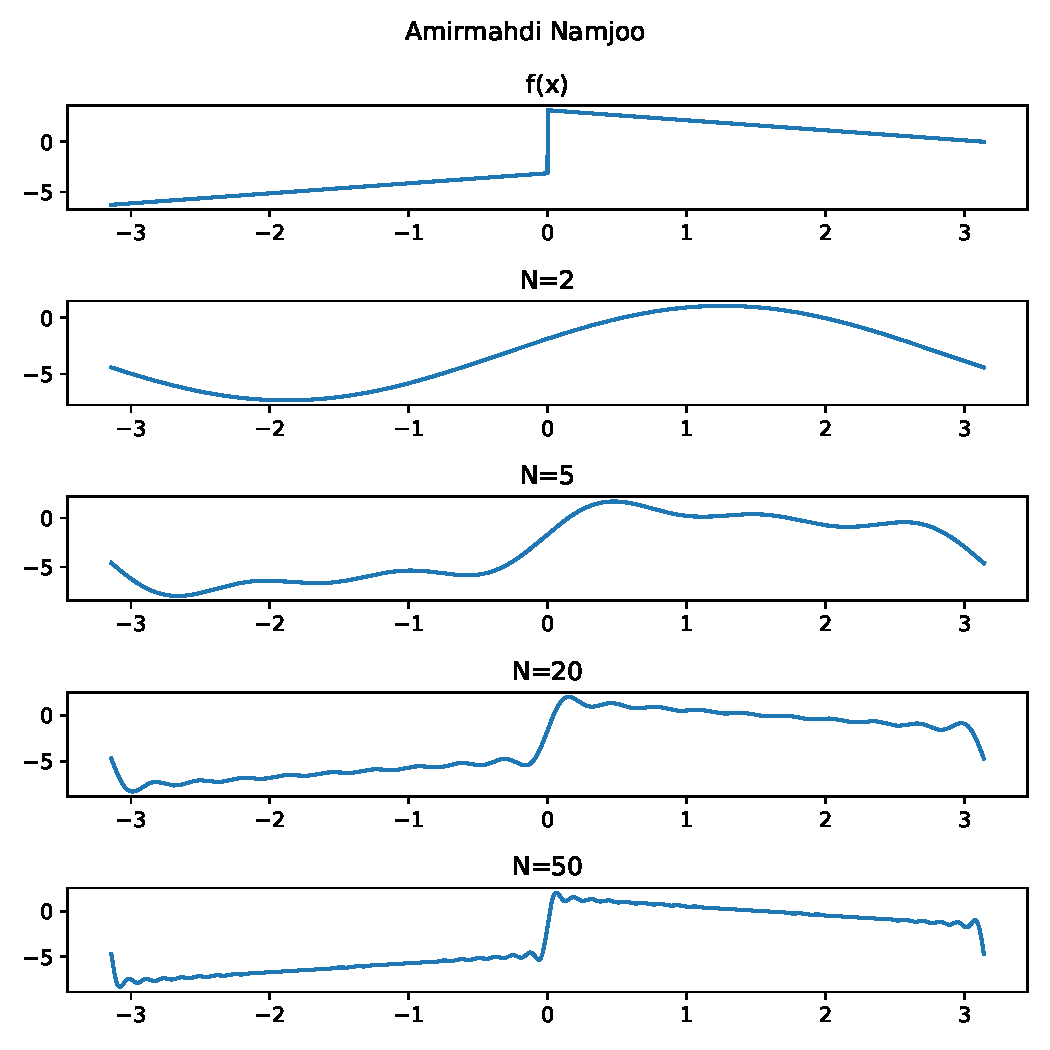
\includegraphics[width = 1.0 \textwidth]{images/1.pdf}
\end{center}


\newpage

\subsubsection{بخش b}

$$
f(x)=\left\{\begin{array}{lr}
	1 & 0 \leq x<\frac{\pi}{2} \\
	0 & \frac{\pi}{2} \leq x<\pi \\
	0 & -\pi \leq x<0
\end{array}\right.
$$

$$a_0 = \frac{1}{2\pi} \int f(x) dx = \frac{1}{2\pi} \int_{0}^{\pi/2} 1 dx = \boxed{ \frac{1}{4}}$$


$$a_n = \frac{1}{\pi} \int (f(x) \cos (nx)) dx$$

$$=\frac{1}{\pi}\int_{0}^{\pi/2} \cos (nx) dx = \frac{1}{\pi }\frac{\sin(nx)}{n}|_{0}^{\pi/2}  = \boxed{\frac{\sin \left(\frac{\pi  n}{2}\right)}{\pi  n}}$$

$$b_n = \frac{1}{\pi} \int (f(x) \sin (nx)) dx$$
$$= \frac{1}{\pi} \int_{0}^{\pi/2} \sin (nx) dx = - \frac{1}{\pi} \frac{\cos (n x)}{n} |_{0}^{\pi/2}  = \boxed{\frac{2 \sin ^2\left(\frac{\pi  n}{4}\right)}{\pi  n}}$$

که در بالا از اتحاد
$\cos(2 \theta) = 1 - 2\sin^2 (\theta)$
استفاده شده است.


و جواب نهایی به صورت:

$$f(x) = a_0 + \sum_{n=1}^{N} (a_n \cos (n x) + b_n \sin (n x))$$



کد آن در فایل 
\lr{\Verb+P1\_Q1\_b.py+}
قرار دارد. نمودار در صفحه بعد قرار گرفته است. شکل بالایی خود تابع و شکل های بعدی به ازای $N=2,5,20,50$ هستند.

\begin{center}
	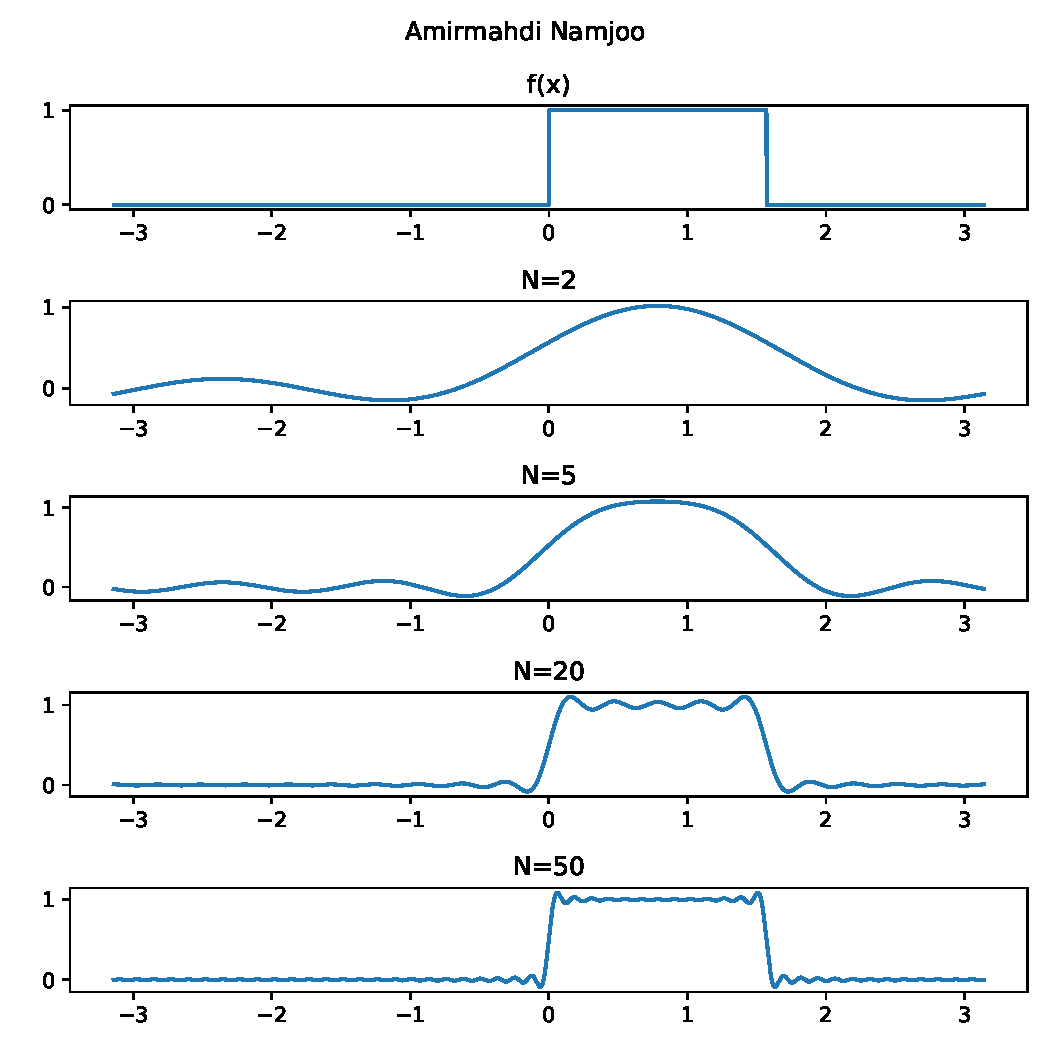
\includegraphics[width = 1.0 \textwidth]{images/2.pdf}
\end{center}

\newpage
\subsection{سوال دوم}
\end{document}



